\documentclass[11pt]{article}
\usepackage[letterpaper,margin=0.85in]{geometry}
\usepackage[T1]{fontenc}
\usepackage[utf8]{inputenc}
\usepackage{lmodern}
\usepackage{microtype}
\usepackage{amsmath,amssymb}
\usepackage{graphicx}
\usepackage{booktabs,tabularx,array}
\usepackage{caption}
\usepackage{fancyhdr}
\usepackage{hyperref}
\usepackage{url}
\usepackage{enumitem}
\hypersetup{colorlinks=true,linkcolor=blue,citecolor=blue,urlcolor=blue}
\captionsetup{labelsep=period,font=small}
\renewcommand{\figurename}{Fig.}
\setlength{\parindent}{0pt}
\setlength{\parskip}{0.45em}
\setlength{\headheight}{14pt}
\pagestyle{fancy}
\fancyhf{}
\fancyhead[L]{\small COMPARATIVE STUDY | REINFORCEMENT LEARNING}
\fancyhead[R]{\small\thepage}
\renewcommand{\headrulewidth}{0.4pt}
\title{A Comparative Study of Deep Reinforcement Learning and\\Counterfactual Regret Minimization in a Simplified Trading Card Game}
\author{Vishva Pujara, Jaimin Sitapara\\[3pt]
\normalsize Department of Computer Science (AI-ML)\\
\normalsize Adani University\\
\small \href{mailto:vishvapujara.cse23@adaniuni.ac.in}{vishvapujara.cse23@adaniuni.ac.in},
\href{mailto:jaiminsitapara.cse23@adaniuni.ac.in}{jaiminsitapara.cse23@adaniuni.ac.in}}
\date{}
\begin{document}
\maketitle
\begin{center}
\large\textit{Completed research project: a custom Pokémon-inspired TCG environment with a 50-dimensional observation vector and 70-action masked action space}
\end{center}
\vspace{-0.5em}


\begin{abstract}

This study compares value-based, policy-gradient, recurrent policy-gradient, and regret-minimization methods in a custom, partially observable, two-player Pok\'emon-inspired card game. The implemented environment uses a 50-dimensional observation vector paired with a separate 70-action legal mask, in a 20-card environment with a two-slot Bench, typed Energy, Retreat, healing, Weakness, knockouts, forced promotion, and deck-out. DQN, PPO, and LSTM-PPO were trained as Red against a legal-random Blue opponent; Deep CFR trained separate Red and Blue networks through external-sampling self-play with a four-step explicit traversal horizon and terminal continuation rollouts. In recorded evaluations, DQN won 72.0\% of 100 games; final PPO and LSTM-PPO won 88.3\% (1,325/1,500) and 88.9\% (1,333/1,500), respectively, against a common 5.7\% legal-random baseline evaluated over 1,500 games. Deep CFR's StrategyNetwork achieved 13.0\% greedily and 9.7\% by sampling, while the distinct policy obtained by regret-matching the learned Red RegretNetwork achieved 53.6\%. A separate 4,000-game head-to-head tournament added 2,400 cross-play games and 1,600 self-play games, with both role orientations for each matchup. In cross-play, PPO recorded 936 wins in 1,200 games (78.0\%), LSTM-PPO 902/1,200 (75.2\%), DQN 451/1,200 (37.6\%), and Deep CFR 111/1,200 (9.2\%). The PPO--LSTM-PPO comparison was close (PPO 211/400, 52.75\%) and was not statistically distinguishable at the 5\% level in a paired-seed analysis. All tournament games terminated within the 200-decision cap, and no illegal actions were recorded. These findings remain descriptive: training protocols were not compute-matched, the tournament used a fixed role-asymmetric game, and deterministic self-play orientation swaps for DQN and both PPO policies replayed identical seed-matched outcomes. Neither the baseline nor tournament results establish equilibrium convergence, exploitability, or general algorithm superiority.

\par\smallskip\noindent\textbf{Keywords:} deep reinforcement learning; trading card games; DQN; PPO; LSTM-PPO; Deep CFR; MCCFR; imperfect-information games

\end{abstract}

\section*{1. Introduction}

Sequential games require agents to choose actions over time while rewards depend on both earlier decisions and another player's behavior. Trading card games make this problem especially concrete: a player chooses among legal actions, observes public board changes and a private hand, and must act without seeing the opponent's hand or future draws. The resulting decision process combines delayed consequences, variable legal actions, stochastic card order, and imperfect information. These properties make card games a useful setting for comparing general-purpose reinforcement-learning methods with algorithms designed for strategic interaction.

Deep Q-Networks (DQN) combine value estimation with replay and a target network, while policy-gradient methods optimize a stochastic policy directly. PPO stabilizes policy updates with a clipped surrogate objective [1, 2]. A recurrent policy can carry information across successive observations, which may help when the current observation omits relevant history; LSTM is a common gated recurrent mechanism for retaining such context [3]. In contrast, counterfactual regret minimization (CFR) and its sampling variants were developed for extensive-form games with imperfect information [4, 5]. Deep CFR replaces tabular regret and strategy representations with function approximation [6].

This paper reports on the completed research project rather than a controlled algorithm benchmark with fully matched training budgets. Its purpose is to compare the observed behavior of four approaches under the implemented game rules and evaluation procedures, while making protocol differences explicit. Results from an earlier 18-observation/18-action prototype are excluded because its observation and action interfaces differ materially from the implemented environment.

\subsection*{Research questions}

\begin{enumerate}[leftmargin=*,label=]

\item RQ1. How did the four implemented algorithms perform against the project's legal-random opponent under their recorded evaluation protocols?

\item RQ2. Did recurrent PPO improve the recorded outcome over feed-forward PPO in this setting?

\item RQ3. How did Deep CFR's learned StrategyNetwork compare with a policy obtained by applying regret matching to the learned RegretNetwork?

\item RQ4. Which features of the environment and experimental design limit cross-algorithm conclusions?

\item RQ5. How do the trained policies perform in role-swapped cross-play and same-family self-play?

\end{enumerate}

\subsection*{Contributions}

The paper (i) specifies the implemented observation, action, information-flow, and terminal rules; (ii) describes the four project-specific training pipelines rather than relying on generic algorithm labels; (iii) consolidates the recorded training and evaluation outcomes while separating sample sizes and policy types; and (iv) identifies limitations, including role asymmetry, a shallow explicit CFR horizon, and incomplete decision-level instrumentation; and (v) adds a 4,000-game role-swapped cross-play and self-play evaluation with per-game outcome records.

\section*{2. Related Work}

DQN demonstrated that a convolutional neural network trained with Q-learning, replay, and a target network could learn control policies from high-dimensional visual input [1]. The present project uses the same broad value-based ingredients but a compact vector observation and explicit legal-action mask. PPO alternates data collection with multiple minibatch updates under a clipped policy objective [2]; here, feed-forward PPO and recurrent PPO share the same game wrapper and evaluation ranges but differ in policy representation and sequence training.

Recurrent neural networks provide a stateful representation of temporal context. LSTM was introduced to improve learning over longer time dependencies by controlling information flow through gated memory cells [3]. LSTM-PPO applies that recurrent representation to actor and critic streams. This design can retain recent observation history, but recurrence alone does not ensure that hidden state is sufficient or that the policy uses it effectively.

CFR minimizes counterfactual regret at information sets in extensive-form games; under the assumptions of the theory, self-play regret minimization supports equilibrium computation [4]. MCCFR samples portions of the game tree, including through external sampling, while retaining regret-update guarantees in expectation for the corresponding sampling formulation [5]. Deep CFR uses neural networks and reservoir sampling to approximate regret and average-strategy learning at scale [6]. Fictitious self-play is another sample-based line of work for imperfect-information games [7]. Those theoretical properties apply to the algorithms and assumptions analyzed in the cited work; they do not automatically transfer to this project's depth-limited, rollout-continued implementation or establish its exploitability.

\section*{3. Environment and Game Design}

The completed research environment is a custom, simplified Pok\'emon-inspired simulation implemented in the project's local game engine, player/deck classes, and Gymnasium-style wrapper; it models a deliberately limited ruleset rather than the full official Pok\'emon TCG. The 20-card deck contains exactly 20 cards per player: one each of Pikachu (Card ID 948), Charmander (926), Swinub (800), and Applin (149); three each of Grass, Fire, Water, and Lightning Energy; and four Potion items. Card identifiers and printed card metadata were checked against the English card-data file supplied on the Pok\'emon Company Kaggle competition data page [8]. The local game rules remain a simplified project implementation, not the restricted competition engine. There is no physical Prize-card pile. An overview of the implemented environment and its principal game mechanics is presented in Fig. 1.

\begin{figure}[!htbp]

\centering

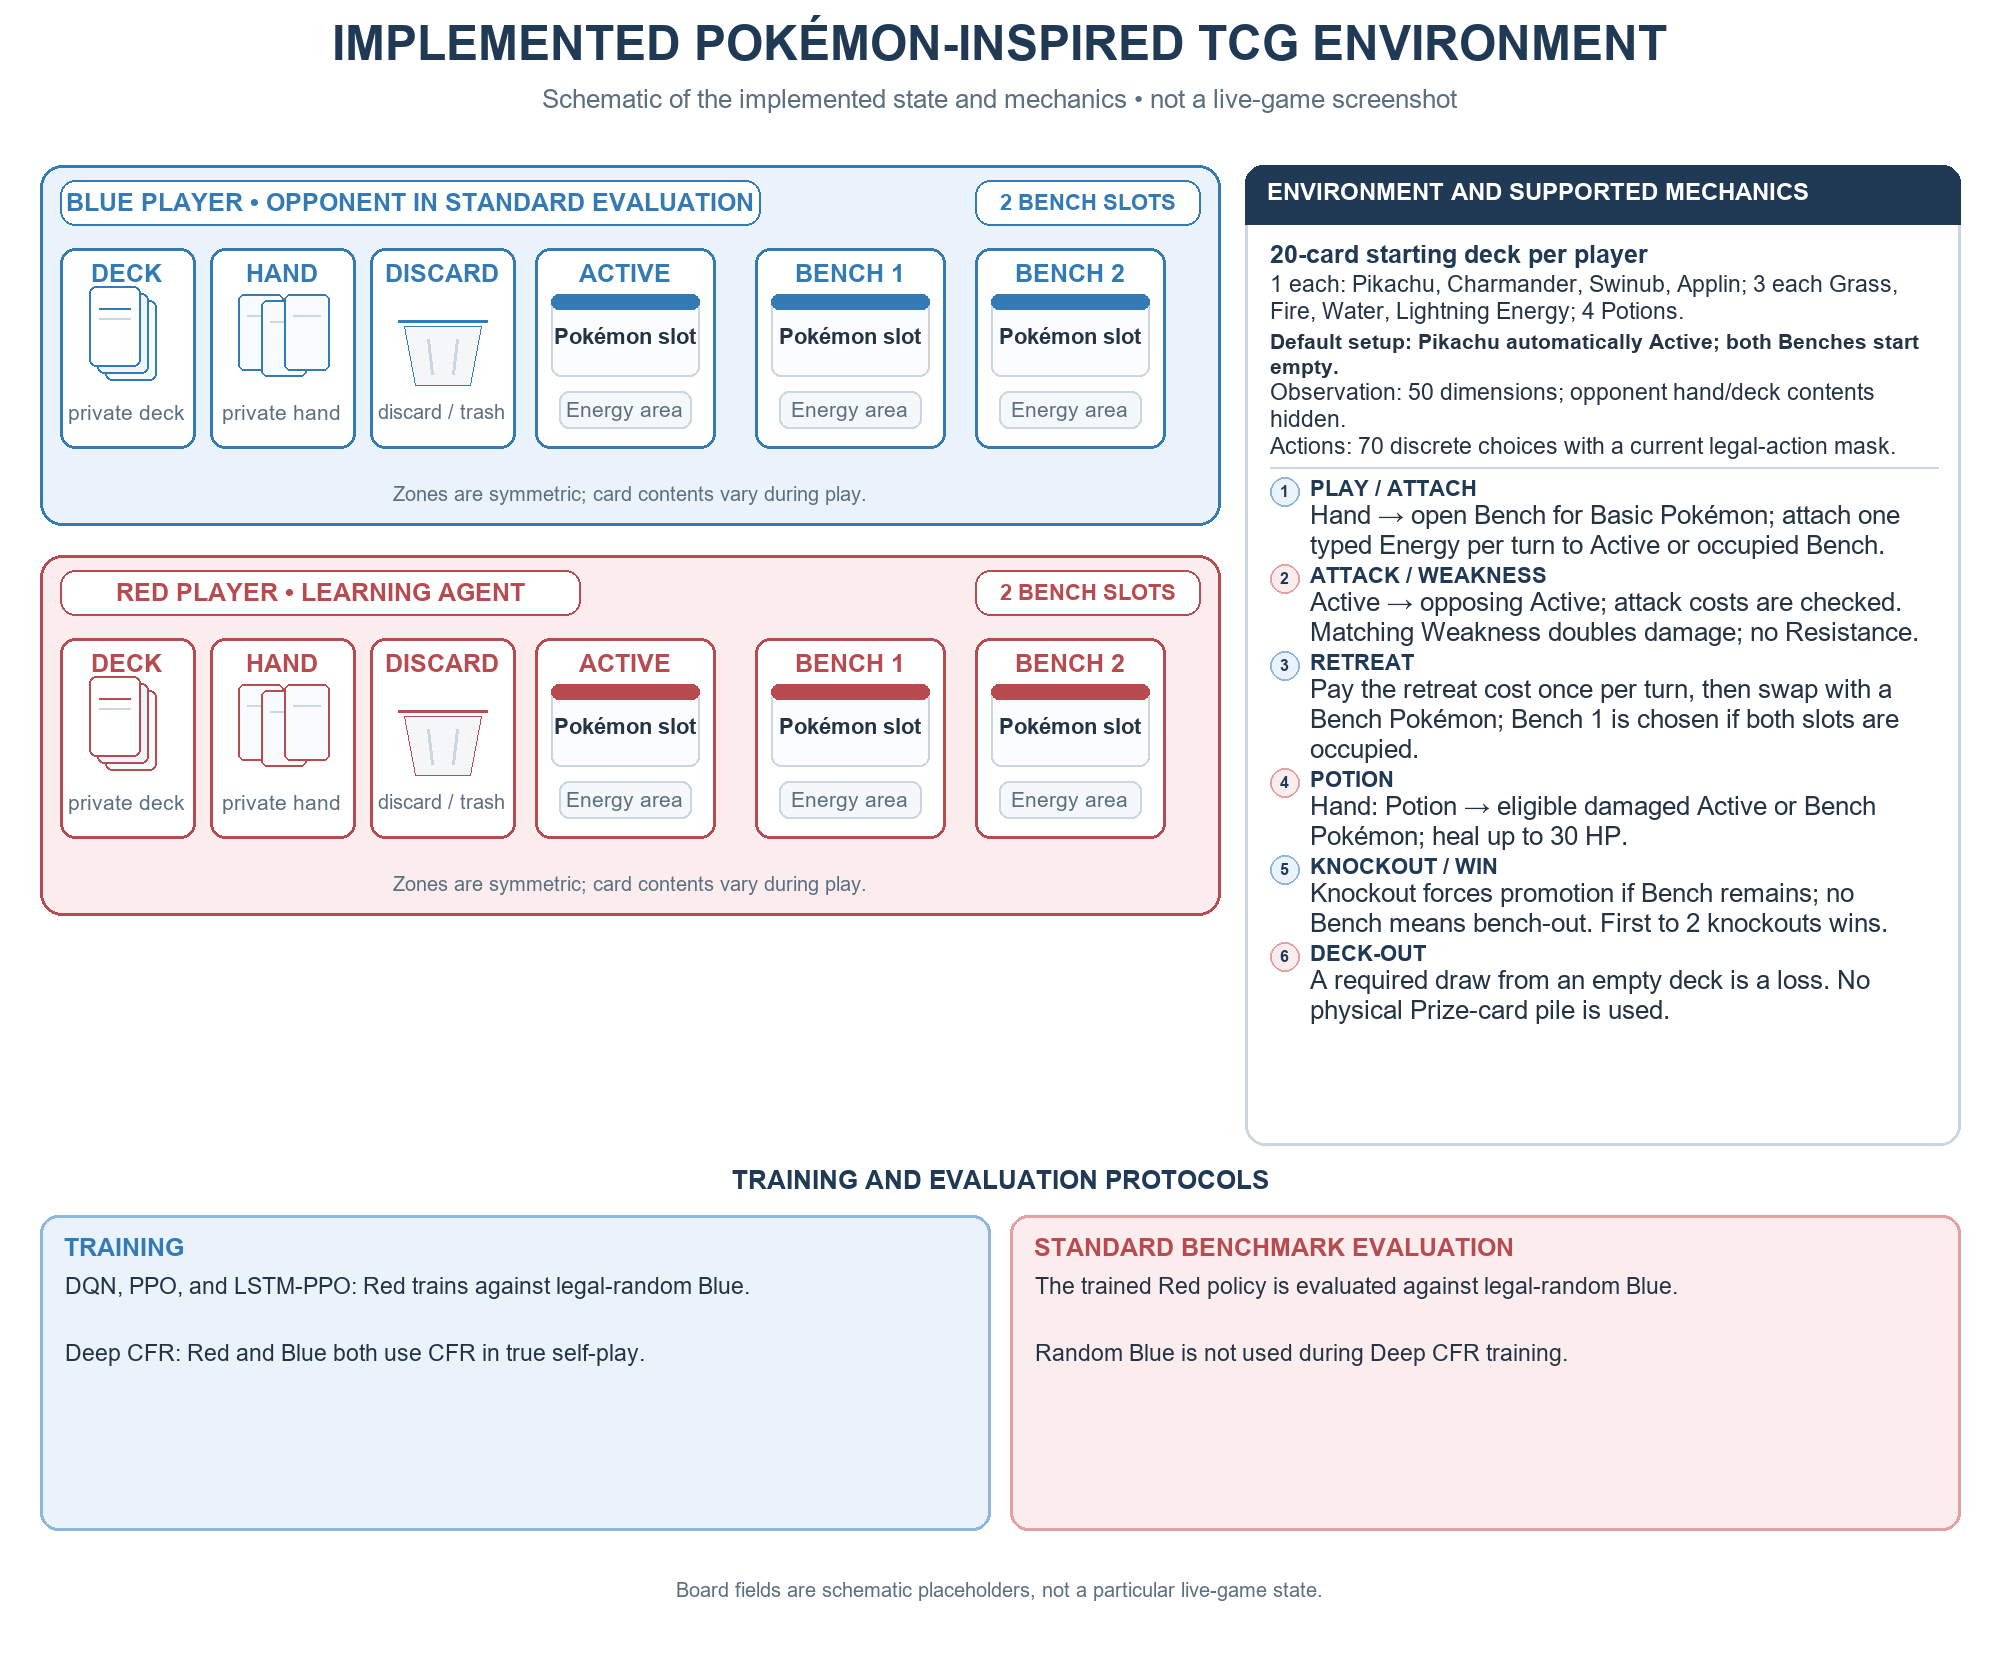
\includegraphics[width=\linewidth,height=0.72\textheight,keepaspectratio]{research_paper/assets/tcg_environment_schematic.png}

\caption{Schematic representation of the implemented Pok\'emon-inspired Trading Card Game environment, illustrating the two-player board, Active Pok\'emon, Bench, deck, hand, Energy attachment, and supported gameplay actions.}

\label{fig:1}

\end{figure}

\begin{table}[!htbp]
\centering
\small
\renewcommand{\arraystretch}{1.12}
\caption{Implemented Pok\'emon profiles and attack costs. Applicable Weakness doubles attack damage; no Resistance rule is present.}
\label{tab:1}
\begin{tabularx}{\linewidth}{>{\raggedright\arraybackslash}X >{\raggedright\arraybackslash}X >{\raggedright\arraybackslash}X >{\raggedright\arraybackslash}X}
\toprule
\textbf{Pok\'emon} & \textbf{HP and type} & \textbf{Weakness / retreat} & \textbf{Implemented attacks} \\
\midrule
Pikachu (948) & 70 / Lightning & Fighting / 1 & Tail Smack: 1 Lightning, 10 damage; Tiny Bolt: 1 Lightning + 1 Colorless, 30 damage \\
Charmander (926) & 80 / Fire & Water / 1 & Fire Claws: 1 Fire + 1 Colorless, 30 damage \\
Swinub (800) & 70 / Water & Metal / 2 & Stampede: 1 Colorless, 10 damage; Icy Snow: 1 Water + 1 Colorless, 20 damage \\
Applin (149) & 40 / Grass & Fire / 1 & Spray Fluid: 1 Grass, 20 damage \\
\bottomrule
\end{tabularx}
\end{table}

\subsection*{3.1 Board, turns, and terminal rules}

Each player has one Active Pok\'emon, a Bench of capacity two, a hand, a draw deck, and a discard/trash area. Basic Pok\'emon can be placed on an empty Bench slot. One Energy may be attached per turn to the Active or an occupied Bench Pok\'emon. Potion heals up to 30 HP and may target an eligible damaged Pok\'emon. Retreat pays the Active Pok\'emon's retreat cost using any attached Energy and exchanges it with a Bench Pok\'emon. If both Bench slots are occupied, the unencoded Retreat target is always Bench 1; if only one is occupied, that Pok\'emon is selected. A Pok\'emon attack checks its Energy cost and damage; matching the defender's Weakness doubles damage. Resistance is not implemented.

A player wins upon causing two opposing Active knockouts. After a knockout, an available Bench Pok\'emon must be promoted; if the defeated player has no Bench, the game ends immediately by bench-out. A player who is required to draw from an empty deck loses immediately. Draws occur during initialization and at turn transitions; The implemented rules include no additional draw effect. Rewards are terminal and zero-sum in the wrapper: Red receives +1 on a Red win and -1 on a Red loss. Evaluation loops impose a maximum of 200 Red-controlled decisions per game; if no Red win is registered by the limit, the evaluator records a non-win/loss.

\subsection*{3.2 Initial state and role asymmetry}

Game initialization scans each configured deck in its existing order and removes the first Pok\'emon encountered for the Active position before shuffling the remaining cards. The configured deck order begins with Pikachu, so both players start with Pikachu Active; this selection is automatic and is not made by the learning agent. The player does not choose a separate opening setup, and both Benches begin empty. The engine then deals three cards to each player and gives Red, the first player, one additional opening card. Red therefore begins with four cards in hand and 15 cards remaining in the deck; Blue begins with three cards and 16 cards remaining. This fixed role and opening-hand asymmetry conditions every reported win rate: Red acts first and receives one extra card. Evaluation seeds control Python's deck-shuffle and environment randomness.

\subsection*{3.3 Information state and privacy}

The network input is a 50-dimensional observation vector built from the observing player's current view. Deep CFR uses this encoded view as its information-state input, but it is a fixed feature representation and is not claimed to be a complete canonical information-set representation. The legal-action mask is a separate binary vector of length 70, recomputed from the current game state; it is not part of the 50 observation values. Indices 0--17 encode the observing player's Active and two Bench slots in three six-value blocks: HP, attached Grass/Fire/Water/Lightning Energy counts, and Pok\'emon type ID. Indices 18--25 encode card-type IDs in that player's first eight visible hand slots; 26 is that player's deck size; 27 indicates whether Energy has been attached this turn; 28 indicates whether Retreat was used; and 29 indicates forced promotion for that player. Indices 30--47 encode the opponent's Active and Bench Pok\'emon using the same six-value blocks. Indices 48 and 49 give opponent hand size and deck size. Empty board slots use all-zero fields; public Pok\'emon type IDs are 0 for absent, 1 Grass, 2 Fire, 3 Water, and 4 Lightning. The opponent's private hand and deck contents are not exposed. The observation builder is symmetric for either player, although the single-agent wrapper exposes Red's view.

\subsection*{3.4 Legal actions and action masks}

The discrete action space has 70 indices. The separate binary legal-action mask is recomputed from the current state and prevents illegal choices, including impossible hand slots and ordinary actions during forced promotion. The fixed mapping is:

\begin{table}[!htbp]
\centering
\small
\renewcommand{\arraystretch}{1.12}
\begin{tabularx}{\linewidth}{>{\raggedright\arraybackslash}X >{\raggedright\arraybackslash}X}
\toprule
\textbf{Indices} & \textbf{Action family} \\
\midrule
0 & End turn \\
1--2 & Attack 1 / Attack 2 \\
3 & Retreat \\
4--11 & Play hand slot 0--7 to Bench 1 \\
12--19 & Play hand slot 0--7 to Bench 2 \\
20--27 & Attach Energy from hand slot 0--7 to Active \\
28--35 & Attach Energy from hand slot 0--7 to Bench 1 \\
36--43 & Attach Energy from hand slot 0--7 to Bench 2 \\
44--51 & Potion from hand slot 0--7 to Active \\
52--59 & Potion from hand slot 0--7 to Bench 1 \\
60--67 & Potion from hand slot 0--7 to Bench 2 \\
68--69 & Promote Bench 1 / Bench 2 \\
\bottomrule
\end{tabularx}
\end{table}

The single-agent interface controls Red and advances an internal legal-random Blue opponent after Red acts. DQN, PPO, and LSTM-PPO therefore train against that random policy. Deep CFR instead traverses and trains both Red and Blue with separate networks during self-play; Random Blue is used only for post-training benchmark evaluation.

\section*{4. Methodology}

\subsection*{4.1 DQN}

The DQN implementation is a 50--128--128--70 multilayer perceptron with ReLU hidden layers and one Q-value per action. Its replay buffer stores state, action, reward, next state, and terminal status, with a 10,000-transition capacity. Epsilon-greedy selection samples uniformly from legal actions during exploration and chooses the highest-valued legal action otherwise. Training uses a separate target network, synchronized every 10 episodes, Adam at 0.0001, discount factor 0.99, batch size 32, and Smooth L1 (Huber) loss. Its one-step target is y$_t$ = r$_t$ + $\gamma$(1 - d$_t$) max$_a$$\in$Alegal(s$_t$$_+$$_1$) Qtarget(s$_t$$_+$$_1$, a). Epsilon starts at 1.0, decays by 0.99 per episode to a minimum of 0.05. The runner creates a fresh 50/70 network and trains for 1,000 episodes, with a 200-step episode cap. The evaluation loads the best rolling-win-rate checkpoint and acts greedily under the legal mask.

\subsection*{4.2 PPO}

PPO uses separate feed-forward actor and critic networks with two 128-unit ReLU hidden layers. The actor outputs 70 logits; a masked categorical distribution assigns zero probability to illegal actions. The critic estimates state value. The clipped surrogate is Lclip = E[min($\rho$$_t$A$_t$, clip($\rho$$_t$, 1 - $\epsilon$, 1 + $\epsilon$)A$_t$)], where $\rho$$_t$ is the new-to-old legal-action probability ratio. Advantages use generalized advantage estimation: $\delta$$_t$ = r$_t$ + $\gamma$(1 - d$_t$)V(s$_t$$_+$$_1$) - V(s$_t$), and A$_t$ = $\delta$$_t$ + $\gamma$$\lambda$(1 - d$_t$)A$_t$$_+$$_1$. Training uses 500 updates of 2,048 Red transitions (1,024,000 total), 10 optimization epochs per update, minibatches of 64, Adam at 0.0001, discount 0.99, GAE lambda 0.95, clipping epsilon 0.2, entropy coefficient 0.01, value coefficient 0.5, and gradient clipping at 0.5. The evaluation policy is greedy over the masked probabilities; the baseline uniformly samples legal actions.

\subsection*{4.3 LSTM-PPO}

LSTM-PPO retains separate actor and critic networks, each with a 50-to-128 dense layer, a 128-unit LSTM, and an output head (70 policy logits for the actor and one value for the critic). It carries actor and critic hidden/cell states across decisions and resets them at episode boundaries. Rollouts are divided into sequences of length 16; recurrent minibatches contain four sequences, and training uses 10 PPO epochs. Its remaining settings are 500 updates of 2,048 transitions (1,024,000 total), learning rate 0.00005, discount 0.99, GAE lambda 0.95, clipping epsilon 0.2, entropy coefficient 0.01, value coefficient 0.5, and gradient clipping at 0.5. Action masks are applied in collection, training, and greedy evaluation. This implementation tests whether recurrent memory helps under the same observation interface; it does not add opponent-hand information.

\subsection*{4.4 Deep CFR}

For legal action a at a traverser decision represented by observation vector o, regret matching uses $\sigma_t(a\mid o) = \frac{R_t^+(o,a)}{\sum_{b\in\mathcal{A}_{\mathrm{legal}}(o)} R_t^+(o,b)}$, where $R^+ = \max(R,0)$; it uses a uniform distribution across legal actions when the denominator is zero. Both players are trained by CFR; Random Blue does not participate in training.

Strategy samples contain a 50-dimensional observation vector, a legal probability target generated by regret matching, its separate action mask, and the current iteration number t. The StrategyNetwork is trained with mask-aware cross-entropy weighted by t: $\mathcal{L} = \frac{\sum_i t_i\,\mathrm{CE}_i}{\sum_i t_i}$, with logits restricted to legal actions. The target distribution itself remains normalized, while each sample's per-state cross-entropy is multiplied by its iteration weight. This is an iteration-weighted sample approximation to the average strategy, not a guarantee of an exact reach-weighted behavioral average at every information set; visits are shaped by traversal and reservoir sampling.

The explicit traversal horizon is four steps. At the boundary the implementation continues the sampled current regret-matching profile until a true terminal outcome and uses that outcome as the continuation value. This avoids assigning an artificial leaf payoff, but still makes the estimator depth-limited and approximate: later decisions are represented by a sampled rollout rather than explicit counterfactual expansion and target collection. Consequently, the run should not be described as exact full-depth MCCFR. Evaluation keeps three policy modes distinct: greedy StrategyNetwork, sampled StrategyNetwork, and direct regret matching over the learned Red RegretNetwork. The last is a diagnostic policy, not the learned average StrategyNetwork.

\begin{figure}[!htbp]

\centering

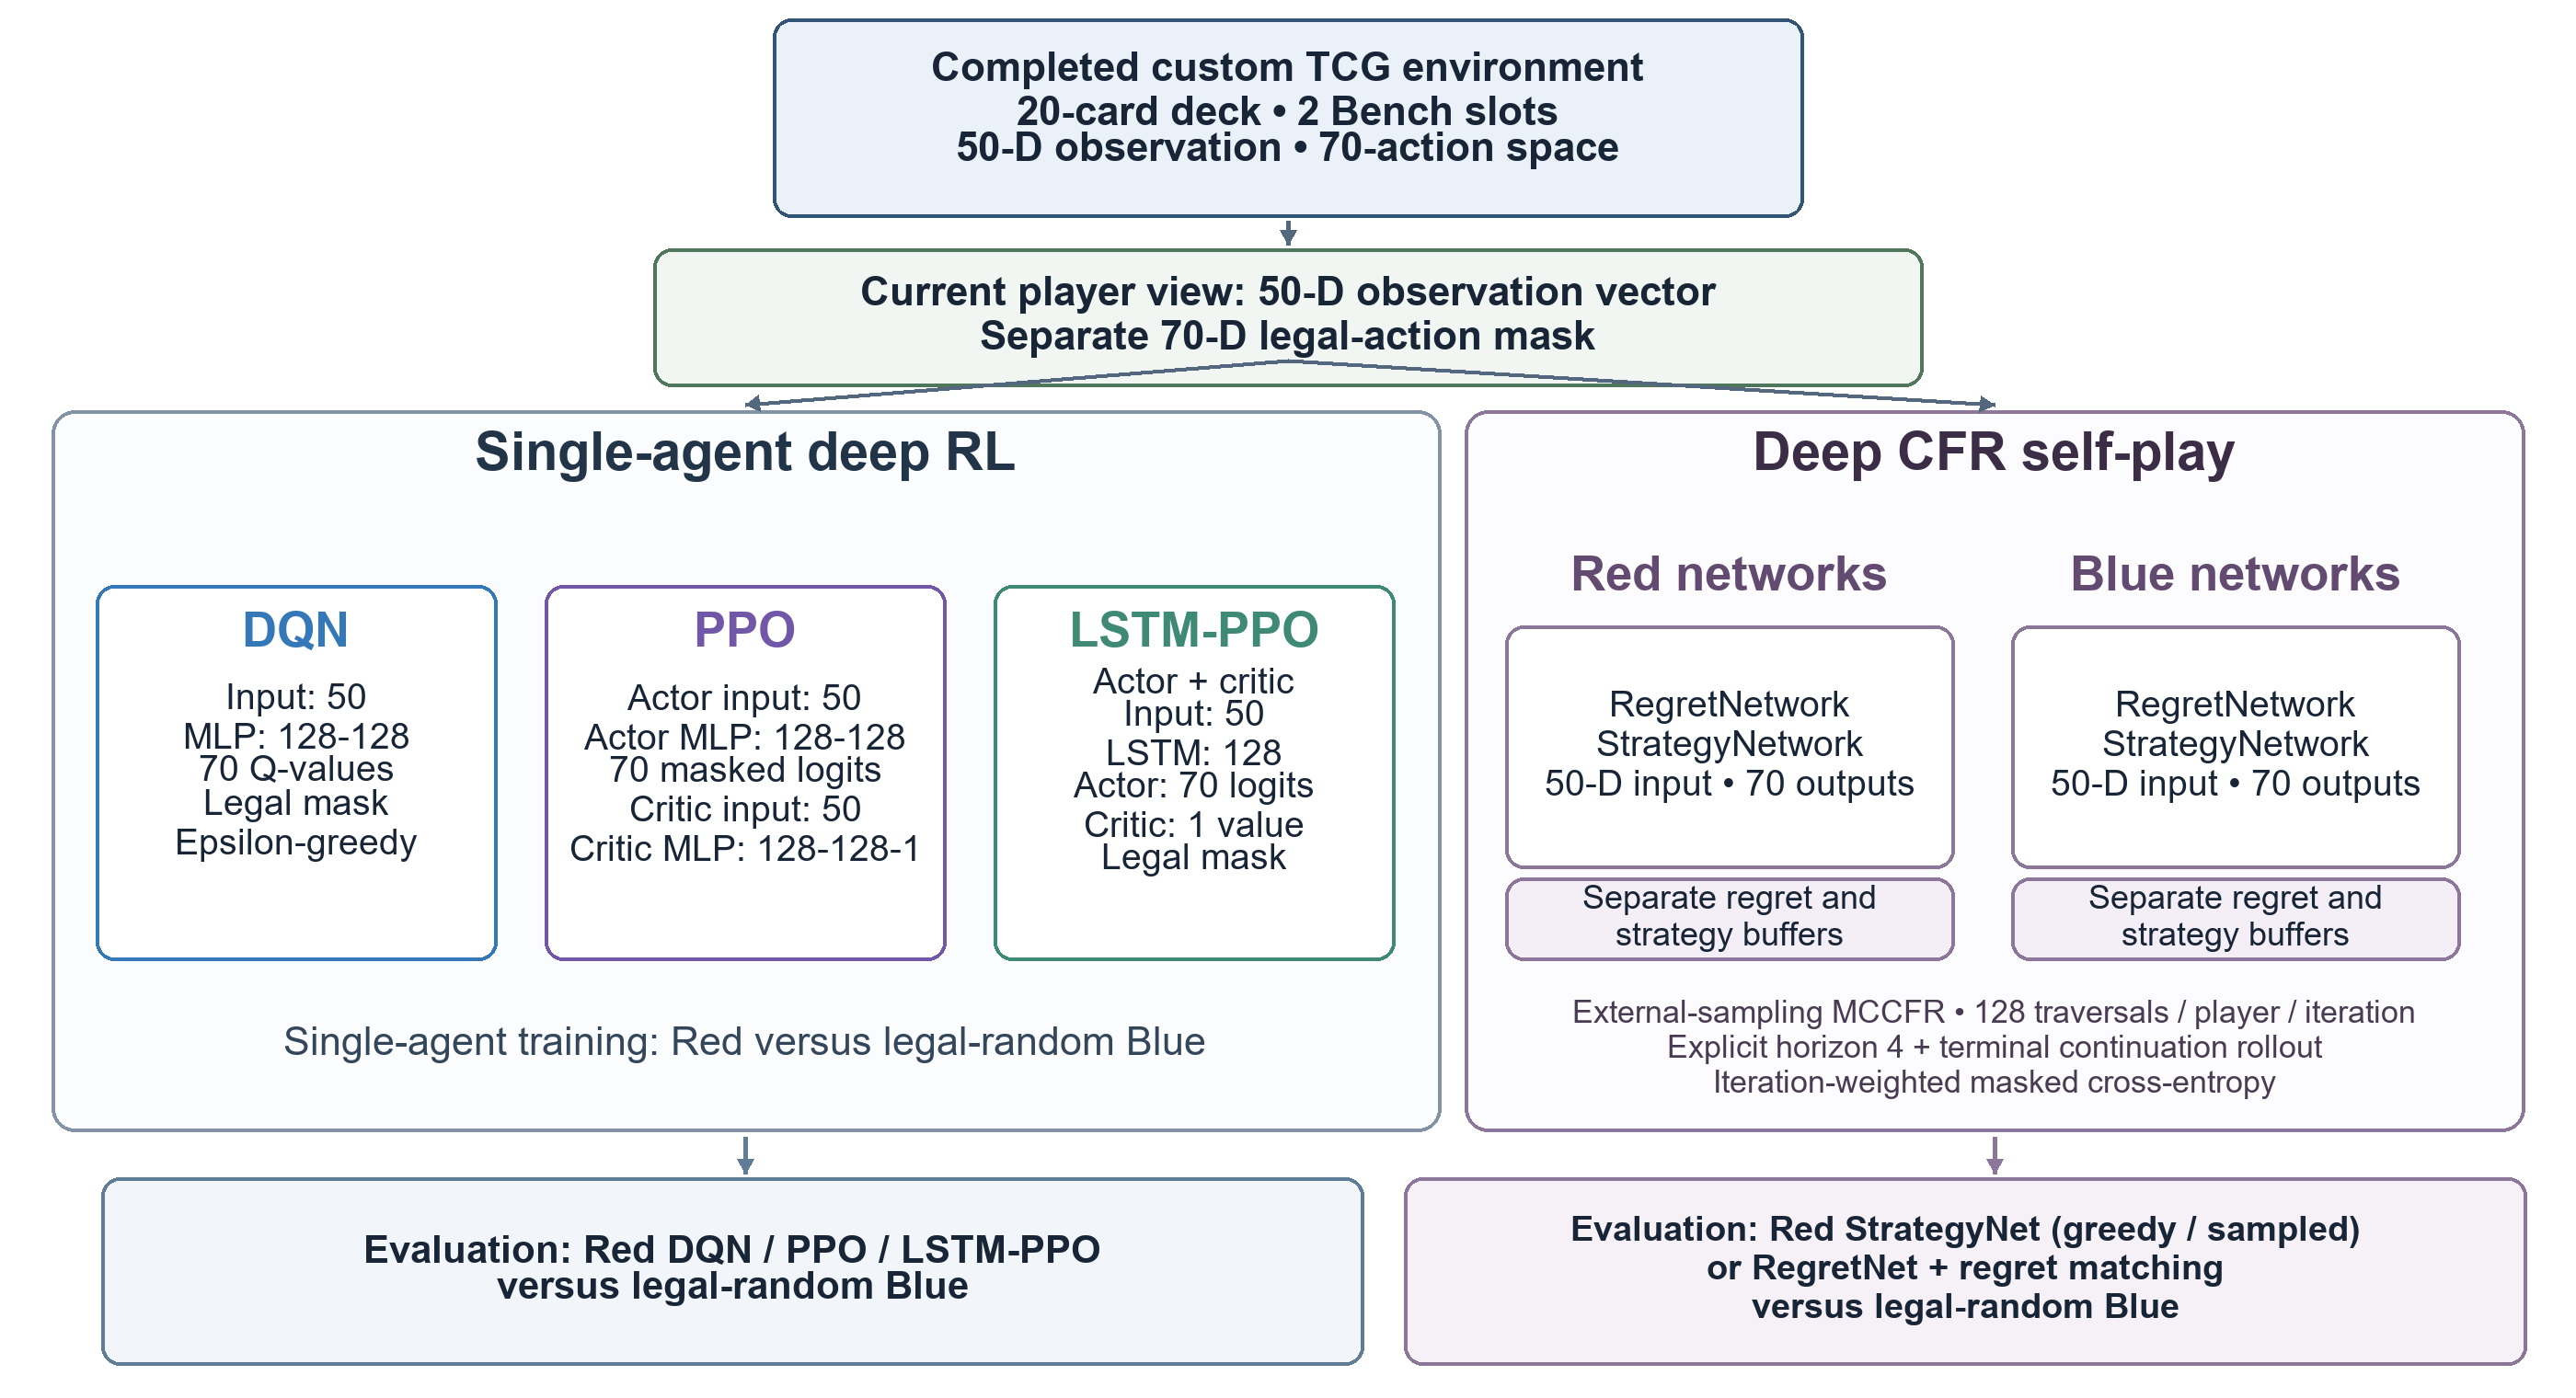
\includegraphics[width=\linewidth,height=0.72\textheight,keepaspectratio]{research_paper/assets/deep_cfr_training_architecture.png}

\caption{Implemented environment, agent, training, and evaluation paths. DQN, PPO, and LSTM-PPO train Red against legal-random Blue; Deep CFR traverses both players with separate networks and is evaluated separately against Random Blue.}

\label{fig:2}

\end{figure}

\section*{5. Experimental Setup}

All main results concern the custom Pok\'emon-inspired TCG environment and its 50-dimensional observation vector with a separate 70-action mask. DQN, PPO, and LSTM-PPO were trained as Red against the wrapper's legal-random Blue policy; Deep CFR used two-player Red/Blue self-play. Training and evaluation seeds were set explicitly by each experiment runner. DQN evaluation used seeds 9999--10098 and 100 games. PPO, LSTM-PPO, and Deep CFR used three 500-game ranges: 10000--10499, 20000--20499, and 30000--30499, for 1,500 games per reported policy. The Random baseline uniformly samples from the current legal-action mask. Trained feed-forward PPO and LSTM-PPO are greedy at evaluation; Deep CFR includes greedy and sampled StrategyNetwork evaluation and a separate regret-matching RegretNetwork diagnostic. Games are capped at 200 Red-controlled decisions. These protocols are not fully matched across algorithms, especially in evaluation size and training objective.

\subsection*{Head-to-head tournament protocol}

After the fixed-opponent benchmark, a separate tournament evaluated the four trained algorithm families directly against one another. The schedule contained six cross-algorithm pairings (DQN--PPO, DQN--LSTM-PPO, DQN--Deep CFR, PPO--LSTM-PPO, PPO--Deep CFR, and LSTM-PPO--Deep CFR), with 200 games in each of the two role orientations, for 2,400 cross-play games. Four same-family matchups (DQN, PPO, LSTM-PPO, and Deep CFR self-play) were also run with 200 games for each instance/role assignment, for 1,600 self-play games. The complete run therefore comprised 4,000 games.

The tournament used the direct game engine so either player could be controlled by a learned policy. Each game was capped at 200 total decisions, counting one engine step by either Red or Blue. The game seed was paired across orientations and matchups (base seed 12345, with 200 game seeds); policy-action random-number generators were independently derived for each game, orientation, seat, algorithm, and player instance. DQN selected the highest-valued legal action with exploration disabled. PPO and LSTM-PPO selected the highest-probability legal action; LSTM-PPO maintained independent recurrent states for the two seats. Deep CFR sampled from the legal, normalized probabilities of its role-specific StrategyNetworks: the Red StrategyNetwork controlled Red and the Blue StrategyNetwork controlled Blue. The regret-matching RegretNetwork diagnostic was not used in this tournament.

The tournament completed all 4,000 games in 108.43 seconds on the reported CUDA device. All games terminated before the cap and no illegal-action attempts were recorded. Terminal outcomes comprised 2,658 two-knockout victories, 831 bench-outs, and 511 deck-outs; all 511 deck-out losses were recorded for Red. Tournament summaries report 95\\% Wilson intervals for orientation-level proportions using terminal games as the denominator. Overall cross-play rankings and Elo are descriptive: the same deck seeds recur across matchups and roles, so pooled game-level Wilson intervals do not account for seed clustering. Elo starts at 1500, uses $K=32$, processes cross-play records in fixed order, and scores capped games as draws (no games were capped).

The experiment machine was reported as an Intel Core Ultra 9 275HX system with 32 GB RAM and an NVIDIA GeForce RTX 5060 Laptop GPU. The experiment's hardware banner reported PyTorch 2.11.0+cu128, CUDA 12.8, and CUDA availability. PPO, LSTM-PPO, and Deep CFR select CUDA when available; the DQN experiment runner also selects the available device for its benchmark run. Hardware/software values are based on the recorded hardware banner and user-supplied machine details; the metric CSVs do not embed a complete reproducibility manifest or package lockfile.

\begin{table}[!htbp]
\centering
\small
\renewcommand{\arraystretch}{1.12}
\begin{tabularx}{\linewidth}{>{\raggedright\arraybackslash}X >{\raggedright\arraybackslash}X >{\raggedright\arraybackslash}X >{\raggedright\arraybackslash}X}
\toprule
\textbf{Algorithm} & \textbf{Training budget} & \textbf{Principal settings} & \textbf{Reported training time} \\
\midrule
DQN & 1,000 episodes; 32,079 recorded Red transitions & Replay 10,000; batch 32; gamma .99; epsilon 1.0 $\rightarrow$ .05 & 342.3 s \\
PPO & 500 $\times$ 2,048 = 1,024,000 steps & 10 epochs; batch 64; lr 1e-4; gamma .99; lambda .95 & 1,956.6 s \\
LSTM-PPO & 500 $\times$ 2,048 = 1,024,000 steps & Sequence 16; 10 epochs; batch 4 sequences; lr 5e-5 & 4,478.3 s \\
Deep CFR & 100 iterations; 12,800 traversals per player & 128/player/iteration; depth 4; batch 128; reservoir 40,000 & 10,737.6 s \\
\bottomrule
\end{tabularx}
\end{table}

\subsection*{Evaluation measures and data provenance}

Win rate is Red wins divided by games. The averages in Tables 3 and 4 come from the project's recorded run summaries available for this revision; the repository contains training-curve CSVs and performance plots but no machine-readable per-game evaluation logs. The plots visibly corroborate the reported win rates, while average-reward and average-length values cannot be independently reconstructed from saved CSV files. DQN's best-checkpoint average reward was not retained and remains NR. DQN nonwins are calculated as games minus wins because its evaluator records wins and reward/length summaries without a separate loss field. Games without a Red win by the 200-decision cap count as nonwins; cap-specific counts were not retained. NR denotes an unavailable metric and is not inferred from win rate.

\section*{6. Results}

\subsection*{6.1 DQN, PPO, and LSTM-PPO}

\begin{table}[!htbp]
\centering
\small
\renewcommand{\arraystretch}{1.12}
\caption{Experimental evaluation against the legal-random Blue policy. DQN uses a 100-game seed protocol; PPO and LSTM-PPO use 1,500 games and the three shared seed ranges. NR means the corresponding evaluation value was not retained in the supplied run summary.}
\label{tab:2}
\begin{tabularx}{\linewidth}{>{\raggedright\arraybackslash}X >{\raggedright\arraybackslash}X >{\raggedright\arraybackslash}X >{\raggedright\arraybackslash}X >{\raggedright\arraybackslash}X >{\raggedright\arraybackslash}X}
\toprule
\textbf{Policy} & \textbf{Games} & \textbf{Wins / nonwins} & \textbf{Win rate} & \textbf{Avg. reward} & \textbf{Avg. length} \\
\midrule
DQN random legal baseline & 100 & 5 / 95 & 5.0\% & -0.90 & 33.7 \\
DQN best checkpoint, greedy & 100 & 72 / 28 & 72.0\% & NR & 20.6 \\
PPO random legal baseline & 1,500 & 86 / 1,414 & 5.7\% & -0.89 & 33.7 \\
PPO best checkpoint & 1,500 & 1,302 / 198 & 86.8\% & +0.74 & 17.3 \\
PPO final checkpoint & 1,500 & 1,325 / 175 & 88.3\% & +0.77 & 17.1 \\
LSTM-PPO best checkpoint & 1,500 & 1,329 / 171 & 88.6\% & +0.77 & 14.6 \\
LSTM-PPO final checkpoint & 1,500 & 1,333 / 167 & 88.9\% & +0.78 & 15.1 \\
\bottomrule
\end{tabularx}
\end{table}

The recorded final PPO and LSTM-PPO checkpoints exceed their shared legal-random baseline by a large margin. Final PPO reports 88.3\% wins, mean reward +0.77, and mean game length 17.1 decisions; final LSTM-PPO reports 88.9\%, +0.78, and 15.1 decisions. LSTM-PPO's final win rate is 0.6 percentage points above PPO's, with a reported mean game length two decisions shorter. The experiment was not designed as a paired statistical comparison, and no confidence intervals or significance tests were recorded; the difference should therefore be treated descriptively. DQN's 72\% result is based on only 100 games with a different seed protocol, so its estimate is less precise and is not directly comparable to the 1,500-game estimates.

\subsection*{6.2 Deep CFR policy evaluations}

\begin{table}[!htbp]
\centering
\small
\renewcommand{\arraystretch}{1.12}
\caption{Deep CFR evaluation on the common 1,500-game seed protocol. The RegretNetwork policy is reported separately from the StrategyNetwork.}
\label{tab:3}
\begin{tabularx}{\linewidth}{>{\raggedright\arraybackslash}X >{\raggedright\arraybackslash}X >{\raggedright\arraybackslash}X >{\raggedright\arraybackslash}X >{\raggedright\arraybackslash}X >{\raggedright\arraybackslash}X}
\toprule
\textbf{Red policy} & \textbf{Games} & \textbf{Wins / nonwins} & \textbf{Win rate} & \textbf{Avg. reward} & \textbf{Avg. length} \\
\midrule
Random legal baseline & 1,500 & 86 / 1,414 & 5.7\% & -0.89 & 33.7 \\
StrategyNetwork, greedy & 1,500 & 195 / 1,305 & 13.0\% & -0.74 & 29.5 \\
StrategyNetwork, sampled & 1,500 & 145 / 1,355 & 9.7\% & -0.81 & 31.1 \\
RegretNetwork + regret matching & 1,500 & 804 / 696 & 53.6\% & +0.07 & 26.6 \\
\bottomrule
\end{tabularx}
\end{table}

\begin{figure}[!htbp]

\centering

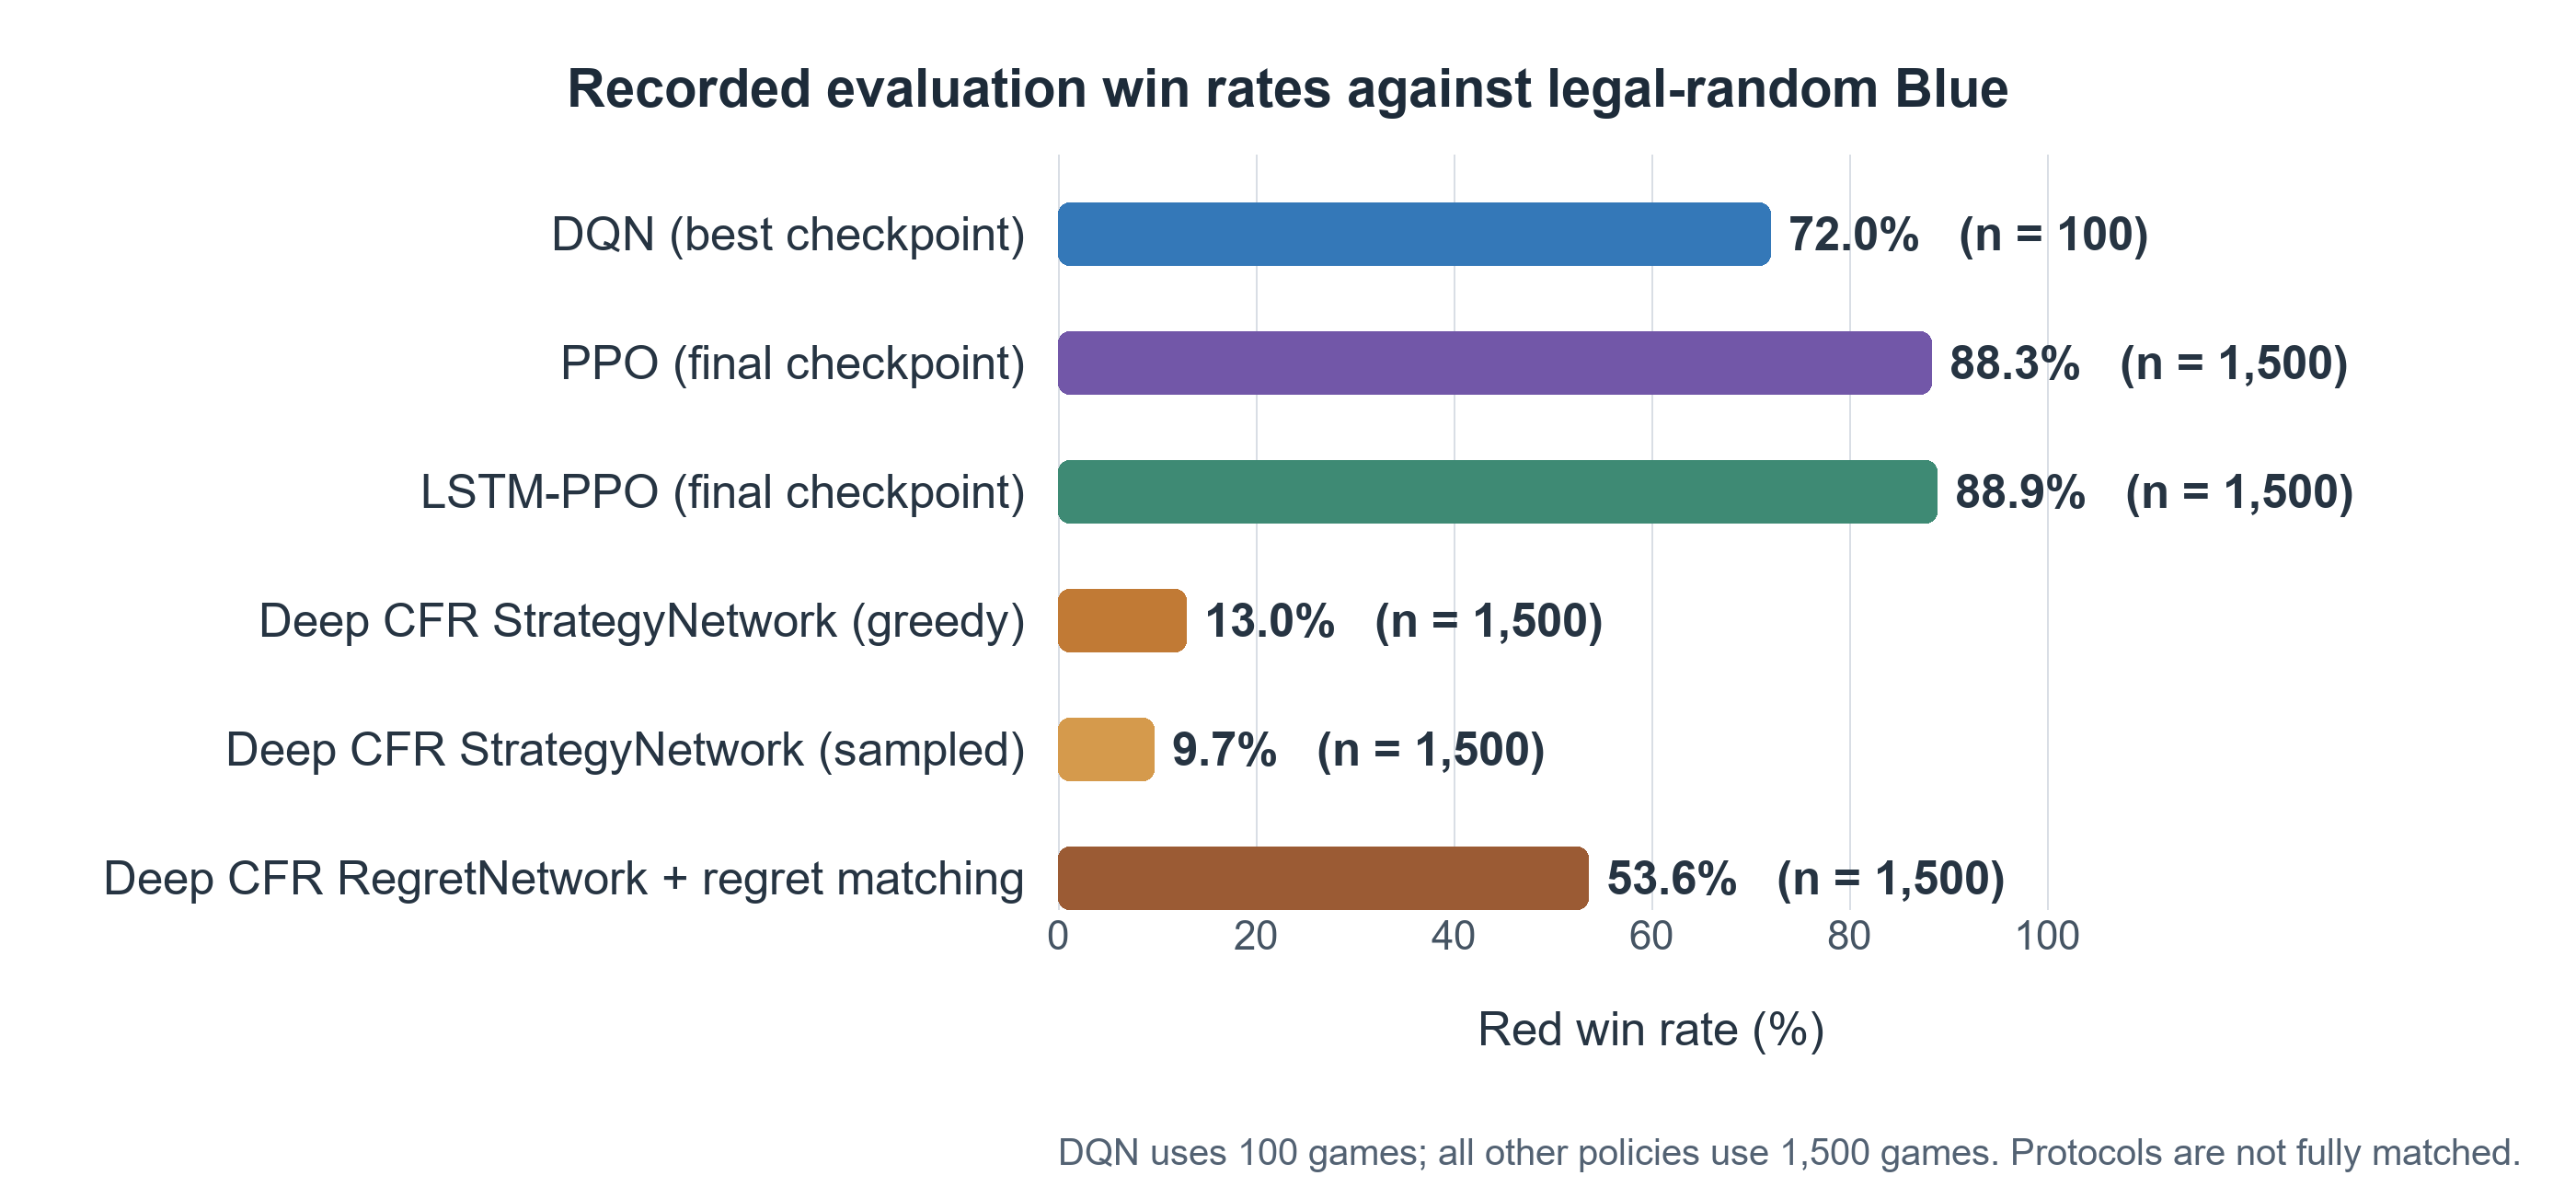
\includegraphics[width=\linewidth,height=0.72\textheight,keepaspectratio]{research_paper/assets/comparative_win_rates.png}

\caption{Recorded Red win rates against legal-random Blue. DQN uses 100 games; every other policy uses 1,500. Sample sizes and training protocols differ, so the bars are descriptive and do not represent a fully matched comparison.}

\label{fig:3}

\end{figure}

The main interpretive result is the separation between policy representations. The StrategyNetwork, trained to approximate the iteration-weighted average strategy, achieved 13.0\% under greedy selection and 9.7\% under action sampling. Applying regret matching directly to the learned Red RegretNetwork achieved 53.6\% against the same Random Blue protocol. This 53.6\% is not the StrategyNetwork's result and should not be reported as average-strategy performance. The discrepancy is consistent with differences between direct regret matching and a separately trained strategy approximation, but these experiments do not isolate a causal explanation. Potential contributors include function-approximation error, state-distribution mismatch, limited traversal coverage, the greedy-versus-sampled decision rule, and training/evaluation opponent mismatch.

\subsection*{6.3 Head-to-head cross-play}

The cross-play results are summarized over both role orientations (200 games per orientation, 400 games per algorithm pairing). The pairwise matrix reports each row algorithm's percentage of completed games won against the column algorithm, pooling the two orientations:

\begin{table}[!htbp]
\centering
\small
\renewcommand{\arraystretch}{1.12}
\caption{Cross-play pairwise win-rate matrix (\%). Each off-diagonal cell pools 400 games across both role orientations; rows identify the algorithm whose win rate is reported.}
\label{tab:4}
\begin{tabularx}{0.9\linewidth}{lrrrr}
\toprule
 & \textbf{DQN} & \textbf{PPO} & \textbf{LSTM-PPO} & \textbf{Deep CFR} \\
\midrule
DQN & --- & 15.8 & 15.8 & 81.2 \\
PPO & 84.2 & --- & 52.8 & 97.0 \\
LSTM-PPO & 84.2 & 47.2 & --- & 94.0 \\
Deep CFR & 18.8 & 3.0 & 6.0 & --- \\
\bottomrule
\end{tabularx}
\end{table}

Across its 1,200 cross-play games, PPO won 936 (78.0\%; 95\% Wilson interval 75.6--80.3\%), LSTM-PPO won 902 (75.2\%; 72.6--77.5\%), DQN won 451 (37.6\%; 34.9--40.4\%), and Deep CFR won 111 (9.2\%; 7.7--11.0\%). The corresponding descriptive Elo ratings were 1768.5, 1592.0, 1568.2, and 1071.3, respectively. These pooled rankings should not be interpreted as compute-matched algorithm rankings: training objectives and budgets differ, the non-CFR policies were trained against legal-random Blue, and Deep CFR was trained through self-play. In addition, the pooled Wilson intervals do not account for the repeated use of paired deck seeds across matchups.

Role-stratified outcomes further demonstrate the importance of seat assignment. PPO won 489/600 games as Red (81.5\%) and 447/600 as Blue (74.5\%); LSTM-PPO won 472/600 as Red (78.7\%) and 430/600 as Blue (71.7\%). DQN won 208/600 as Red (34.7\%) and 243/600 as Blue (40.5%). Deep CFR won 29/600 as Red (4.8\%) and 82/600 as Blue (13.7\%). The Deep CFR seat comparison also reflects the use of distinct role-specific Red and Blue StrategyNetworks, not only the first-player rule.

PPO won 211 of the 400 PPO--LSTM-PPO cross-play games (52.75\%). Its ordinary Wilson interval was 47.9--57.6\%. The paired-seed analysis found 24 seed pairs in which PPO won both orientations, 13 in which LSTM-PPO won both, and 163 split pairs; the paired exact sign test gave $p\\approx0.099$. The estimated difference was therefore not statistically distinguishable from 50\\% at the 5\\% level. This tournament does not support a claim that PPO is superior to LSTM-PPO in their direct matchup.

\subsection*{6.4 Self-play outcomes and replication diagnostic}

Each same-family self-play condition contained 200 games per instance/role assignment. DQN self-play produced 98 Red wins and 102 Blue wins in each orientation (mean 48.0 decisions/game). PPO self-play produced 122 Red wins and 78 Blue wins in each orientation (36.8 decisions/game). LSTM-PPO self-play produced 115 Red wins and 85 Blue wins in each orientation (36.0 decisions/game). Deep CFR self-play produced 52 Red wins and 148 Blue wins in the first assignment, and 56 Red wins and 144 Blue wins in the swapped assignment (approximately 54.5 decisions/game). Deep CFR's Red and Blue players use different role-specific StrategyNetworks; the observed seat split therefore combines role asymmetry and policy-network differences. None of these same-family outcomes measures equilibrium quality or exploitability.

A post-run comparison of the per-game records revealed that the two orientation rows for DQN, PPO, and LSTM-PPO self-play reproduced identical recorded outcomes for all 200 matched seeds in each policy family. These agents load the same shared checkpoint independently for both seats and use deterministic action selection; swapping instance labels does not change the policy assigned to either seat. Thus, the two orientation rows are not 400 independent self-play trajectories for these three methods. The second row is a replay of the same seed-matched outcomes to high confidence; action traces were not saved, so exact step-by-step identity could not be checked. Deep CFR did not show this pattern: its two role-specific StrategyNetworks and sampled actions produced matching outcome tuples for only 4 of 200 seed pairs. Self-play summaries are consequently reported by orientation and are not pooled as independent replications.

\subsection*{6.5 Exploratory StrategyNetwork coverage diagnostic}

A separate, small diagnostic used 10 training iterations, 16 traversals per player per iteration, depth four, iteration-weighted masked cross-entropy, and 200 evaluation games. Exact observation-plus-action-mask hash matching covered 75 of 6,043 unique greedy-evaluation states (1.24\%) and 76 of 6,405 unique sampled-evaluation states (1.19\%). Coverage after the fourth game decision was effectively zero in that pilot. These values describe only the pilot's exact-hash match rate; they do not establish coverage for the full 100-iteration checkpoint and do not prove that coverage caused its evaluation results.

\section*{7. Discussion}

The separate head-to-head tournament adds a different view: PPO and LSTM-PPO won most of their cross-play games, while DQN had a mixed record and the role-specific Deep CFR StrategyNetwork policies won a smaller share against these particular opponents. This does not contradict the earlier Random-opponent benchmark; the opponent populations and seat protocols differ. The direct PPO--LSTM-PPO result was close and not statistically significant under the paired-seed test. The deterministic self-play replication finding also means that the two seat-assignment rows for DQN, PPO, and LSTM-PPO must not be counted as independent duplicate evidence.

The highest recorded win rates in this project were produced by final PPO and LSTM-PPO against the fixed legal-random opponent. This observation is specific to one custom environment, a fixed Red role, and the recorded protocols; it is not evidence that PPO-family methods dominate regret minimization in imperfect-information games generally. The results show that methods optimized directly against this opponent can perform well under the distribution used for training and evaluation. Deep CFR has a different objective: it performs two-player self-play, and evaluation against Random Blue measures response to one opponent rather than equilibrium quality.

The low Random baseline is also role-conditioned. Red starts first and receives one extra card, yet random legal action selection wins only about 5--6\% in the reported game. It is therefore not meaningful to compare this value with a nominal 50\% chance rate. Game outcomes are affected by the custom deck composition, setup, draw and deck-out rules, action semantics, and the deterministic role assignment. A role-swapped evaluation would be required to separate first-player advantage from policy strength.

The RegretNetwork/StrategyNetwork gap is particularly useful diagnostically. The average-strategy head is a learned approximation trained from stored strategy targets with iteration-weighted masked cross-entropy; the regret-matching policy transforms the RegretNetwork's outputs at decision time. They are different functions with different error modes. The StrategyNetwork may fail to reproduce the distribution induced by regret matching away from sampled states, while argmax can further change a stochastic policy. Yet sampled StrategyNetwork performance is also low, so greediness alone is not a sufficient explanation. The small coverage pilot raises a possible generalization concern but cannot be generalized to the full training run.

The CFR implementation's four-step explicit horizon and terminal continuation reduce the amount of explicit tree expansion, but introduce approximation and rollout variance. Continuation values depend on the current regret-matching profile and sampled future trajectory. Information sets beyond the explicit horizon do not contribute the same explicit regret and strategy target coverage as expanded nodes. Same-turn setup decisions such as playing Pok\'emon, attaching Energy, and using items can consume substantial depth before attacks or terminal outcomes occur. As a result, horizon four may underrepresent strategically important later decisions. The supplied study did not run controlled horizon comparisons at equal compute, estimate exploitability, or calculate confidence intervals.

\section*{8. Limitations and Threats to Validity}

First, the environment is a compact custom simulation with a small fixed card pool and simplified rules; results do not transfer directly to the official Pok\'emon TCG or other games. Second, Red and Blue have fixed roles and unequal initial hand sizes: Red acts first and receives one additional opening card. The tournament balances the number of appearances in each seat, but does not remove the underlying role asymmetry. All 511 deck-out losses in the tournament were Red losses, consistent with Red beginning with fewer cards remaining in its deck; this observed association should be interpreted in the context of the implemented draw rules.

Third, training protocols differ: DQN is episode-based and its earlier Random-opponent evaluation used 100 games, PPO-family methods are trained for 1.024 million Red decisions and evaluated for 1,500 Random-opponent games, and Deep CFR uses 100 self-play iterations with sampled traversals. Wall-clock times and training budgets are not controlled for equal compute or sample counts. Fourth, the earlier benchmark evaluates against a single legal-random opponent, whereas the tournament uses the four trained policy families; neither provides a broad external opponent suite.

Fifth, tournament deck seeds are paired across matchups, so pooled game-level Wilson intervals for algorithm rankings do not account for seed clustering. The PPO--LSTM-PPO comparison used a paired-seed test and did not reach the 5\\% significance threshold. Sixth, the tournament retained per-game outcome records but not action-by-action traces. The DQN, PPO, and LSTM-PPO self-play seat-swap conditions reproduced identical recorded outcomes for all 200 matched seeds per family, so their duplicated orientation rows must not be treated as independent replications. Finally, Deep CFR remains depth-limited with rollout continuation and a neural approximation of its strategy average. The exploratory coverage pilot used only 10 iterations and 200 evaluation games, so its low exact-hash match rate is not evidence about the full run by itself.

\section*{9. Future Work}

Future work should add stochastic policy variants and independent policy seeds to determine whether the deterministic self-play replication finding generalizes beyond the current checkpoints. Per-decision action traces would enable trajectory-level audits and analyses of action distributions throughout a game. Further evaluation should use a broader opponent suite, additional independently generated deck seeds, and seed-clustered or paired statistical procedures. A controlled Deep CFR study should compare explicit traversal horizons and continuation policies under matched compute budgets. Where the game representation supports reliable analysis, exploitability or related strategic-quality measures should complement empirical win rates. These are proposed experiments; they were not conducted in the present study.

\section*{10. Conclusion}

This paper presented a comparison of DQN, PPO, LSTM-PPO, and Deep CFR in a custom Pok\'emon-inspired TCG environment with a 50-dimensional observation vector and 70-action masked interface. In the earlier legal-random benchmark, final PPO and LSTM-PPO achieved win rates of 88.3\\% and 88.9\\%, respectively; the 0.6-percentage-point difference was descriptive. A subsequent 4,000-game tournament evaluated cross-play and self-play. PPO recorded the highest pooled cross-play score (78.0\\%), followed by LSTM-PPO (75.2\\%), DQN (37.6\\%), and Deep CFR (9.2\\%) against the specific policy mix and role schedule used. The direct PPO--LSTM-PPO comparison was not statistically distinguishable at the 5\\% level. The self-play audit identified duplicated deterministic trajectories for the two seat assignments of DQN, PPO, and LSTM-PPO, limiting the independent evidence from those rows. Deep CFR's earlier StrategyNetwork and RegretNetwork evaluations also remain distinct policy results. Taken together, the experiments describe how these particular trained checkpoints behaved under the implemented rules and protocols; they do not establish Nash equilibrium, low exploitability, or general superiority of any algorithm.

\section*{References}

\begin{thebibliography}{8}

\bibitem{ref1} V. Mnih et al., ``Human-level control through deep reinforcement learning,'' Nature, vol. 518, no. 7540, pp. 529--533, 2015, doi: 10.1038/nature14236.

\bibitem{ref2} J. Schulman, F. Wolski, P. Dhariwal, A. Radford, and O. Klimov, ``Proximal Policy Optimization Algorithms,'' arXiv:1707.06347, 2017, doi: 10.48550/arXiv.1707.06347.

\bibitem{ref3} S. Hochreiter and J. Schmidhuber, ``Long Short-Term Memory,'' Neural Computation, vol. 9, no. 8, pp. 1735--1780, 1997, doi: 10.1162/NECO.1997.9.8.1735.

\bibitem{ref4} M. Zinkevich, M. Johanson, M. Bowling, and C. Piccione, ``Regret Minimization in Games with Incomplete Information,'' in Advances in Neural Information Processing Systems, vol. 20, 2007, pp. 1729--1736. [Online]. Available: \url{https://proceedings.neurips.cc/paper_files/paper/2007/hash/08d98638c6fcd194a4b1e6992063e944-Abstract.html}.

\bibitem{ref5} M. Lanctot, K. Waugh, M. Zinkevich, and M. Bowling, ``Monte Carlo Sampling for Regret Minimization in Extensive Games,'' in Advances in Neural Information Processing Systems, vol. 22, 2009, pp. 1078--1086. [Online]. Available: \url{https://proceedings.neurips.cc/paper_files/paper/2009/hash/00411460f7c92d2124a67ea0f4cb5f85-Abstract.html}.

\bibitem{ref6} N. Brown, A. Lerer, S. Gross, and T. Sandholm, ``Deep Counterfactual Regret Minimization,'' in Proc. 36th Int. Conf. Machine Learning, PMLR, vol. 97, 2019, pp. 793--802. [Online]. Available: \url{https://proceedings.mlr.press/v97/brown19b.html}.

\bibitem{ref7} J. Heinrich, M. Lanctot, and D. Silver, ``Fictitious Self-Play in Extensive-Form Games,'' in Proc. 32nd Int. Conf. Machine Learning, PMLR, vol. 37, 2015, pp. 805--813. [Online]. Available: \url{https://proceedings.mlr.press/v37/heinrich15.html}.

\bibitem{ref8} The Pok\'emon Company -- PTCGABC Team, ``The Pok\'emon Company -- PTCG AI Battle Challenge Strategy,'' Kaggle dataset, 2026. [Online]. Available: \url{https://www.kaggle.com/competitions/pokemon-tcg-ai-battle-challenge-strategy/data}. Accessed: Nov. 3, 2026. Card-data access and use are subject to the associated competition rules.

\end{thebibliography}

\end{document}
